\documentclass[12pt]{article}
\setlength{\oddsidemargin}{0in}
\setlength{\evensidemargin}{0in}
\setlength{\textwidth}{6.5in}
\setlength{\parindent}{0in}
\setlength{\parskip}{\baselineskip}

\usepackage{amsmath,amsfonts,amssymb}
\usepackage{graphicx}
\usepackage{fancyhdr}
\usepackage{tikz}
\usetikzlibrary{arrows, calc}
\pagestyle{fancy}


\begin{document}

\rhead{{\bf CSCI 3104 \\Problem Set 9\\ Spring 2017, CU-Boulder}}
\lhead{{\bf 
        Grant Baker (07/23) \\ 
        Sam Cuthbertson (06/16)\\ 
        Connor Hudson (05/07)}}
\renewcommand{\headrulewidth}{0.4pt}
\headheight = 43pt


\vspace{-3mm}
\begin{enumerate}

% 	\item (60 pts) Recall that a simple breadth-first search algorithm can be used to solve the All Pairs Shortest Paths (APSP) problem for a simple graph $G=(V,E)$. When $G$ is given in an adjacency list format, this takes both $O(V+E)$ time and space. Across all pairs $i,j\in V$, the shortest path with the longest length is called the \textit{diameter}, and the average length across all such paths is called the \textit{mean geodesic distance}.
	
% 	In this problem, we will implement and apply four functions.
	
% 	(i) {\tt computeDistances(G,s)} takes as input a simple graph $G=(V,E)$ in an adjacency list format and a node $s\in V$, and it returns a vector containing the length of the shortest paths from $s$ to all nodes $t\in V-s$ \textit{and} a tuple containing the number of atomic operations and the maximum length of the queue it took to compute this vector. Nodes that are unreachable from $s$ should be given a special infinite distance value.

% 	(ii) {\tt largestComponentSize(G)} takes as input a simple graph $G=(V,E)$ in an adjacency list format and returns the size of the largest component in $G$ as an integer.
	
% 	(iii) {\tt howBigIsThisGraph(G)} takes as input a simple graph $G=(V,E)$ in an adjacency list format and returns two tuples, one containing the diameter and the mean geodesic distance of $G$, and one containing the number of atomic operations and the maximum length of the queue it took to compute the first tuple. This function should call {\tt computeDistances(G,s)}. When you calculate the diameter and mean geodesic distance, drop any terms that represent an infinite distance.
	
% 	(iv) {\tt erdosRenyiGraph(n,c)} takes as input two positive integers $n$, the number of nodes in the graph, and $c$, the average degree of a node, and returns a simple graph $G=(V,E)$, in adjacency list format, such that $|V|=n$ and $\forall_{i>j} \, (i,j)\in E$ with probability $c/(n-1)$. (Don't forget to add $(j,i)$ to $E$ to make the graph undirected.) This kind of a graph is called an Erd\"os-R\'enyi random graph.
	
% 	\begin{enumerate}
% 	\item From scratch, implement the functions {\tt computeDistances}, {\tt largestComponentSize}, {\tt howBigIsThisGraph}, and {\tt erdosRenyiGraph}. You may not use any library functions that make their implementation trivial. 

% 	Submit (i) a brief explanation for each function that explains how you implemented it (describe how it works and how it uses its data structures), and (ii) your code implementation, with code comments. \label{q:bfs:code}

% 	\item Letting $c=5$ and $n=2^{k}$ for all integers $4\leq k \leq 12$ for the function call {\tt howBigIsThisGraph(  erdosRenyiGraph(n,c) )}, produce a single nice figure showing how both the \textit{diameter} and the \textit{mean geodesic distance} vary as a function of $n$. Include on your figure a line showing the asymptotic behavior of the way these quantities vary with $n$. State the asymptotic relationship. No credit if axes are unlabeled or if the three lines on the figure are unlabeled.
	
% 	Hint: you will get a smoother line if you run the code several times for each $k$ and then instead plot the average value of the diameter or mean geodesic distance. \label{q:bfs:diameter}

% 	\item For the same choices of $c$ and $k$ above, produce two nice figures, one showing the running time and and one showing the space usage. Include on your figure a line showing the asymptotic behavior of the resource usage, and comment on whether it agrees with our analysis in lecture. No credit if axes or lines on the figure are unlabeled.
	
% 	\item Letting $n=500$ and $c=k/5$ for all integers $0\leq k \leq 25$, use the function call {\tt largestComponentSize( erdosRenyiGraph(n,c) )} to obtain the data necessary to make a nice figure showing how the size of the largest component varies with the mean degree. No credit if axes or lines on the figure are unlabeled.
	
% 	You should see something surprising on your plot! What you should see is a \textit{phase transition}, of the same kind that happens in physics, e.g., when water boils into vapor or when a ferric metal suddenly becomes magnetic. Below a \textit{critical value} of $c$ (which value does it look like on your plot?), the size of the largest component is \textit{independent} of the size of the graph, containing $\Theta(1)$ vertices, while above that value, they are proportional, so that the largest component contains $\Theta(n)$ vertices. The transition between these two behaviors occurs suddenly, as a function of the mean degree $c$. This behavior is why, in some complex systems, making things more interconnected can produce sudden changes in system behavior.
	
% 	\item (10 pts extra credit) Using the data file on the class Moodle and your functions above, compute the diameter and the mean geodesic distance. This file contains a snapshot of the Facebook friendship network at a major U.S.\ university from 2005, when Facebook was only open to students, faculty, staff and alumni of about 100 select colleges and universities. Using the diameter and mean geodesic results for this graph, and your figure from part~\eqref{q:bfs:diameter}, roughly estimate via extrapolation what the diameter and mean geodesic distance should be today, now that Facebook claims about $n=10^{9}$ users. Discuss why the value of your rough estimate is or is not surprising to you in any way, and what it might mean for how information travels across Facebook.
	
% 	\end{enumerate}
% 	{\sf Guess I'll grab this -C}
	\addtocounter{enumi}{1}
	\item \textit{(30 pts total) Hagrid, the half-giant gamekeeper at Hogwarts, has installed a set small canals that convey water from a spring in the Forbidden Forest $s$ to his house $t$. (He couldn't install just one big canal for some vague reason having to do with the Forbidden Forest getting mad about it.) Now, he's considering adding a new canal connecting the spring to his directed distribution network $G$. However, he's not sure how much additional water he will be able to push through $G$ after adding the proposed canal. Hagrid needs your help to figure it out. The diagram below shows $G'$, the network $G$ plus the proposed canal $X$; edge labels indicate edge capacities.}
	
	\begin{center}
	    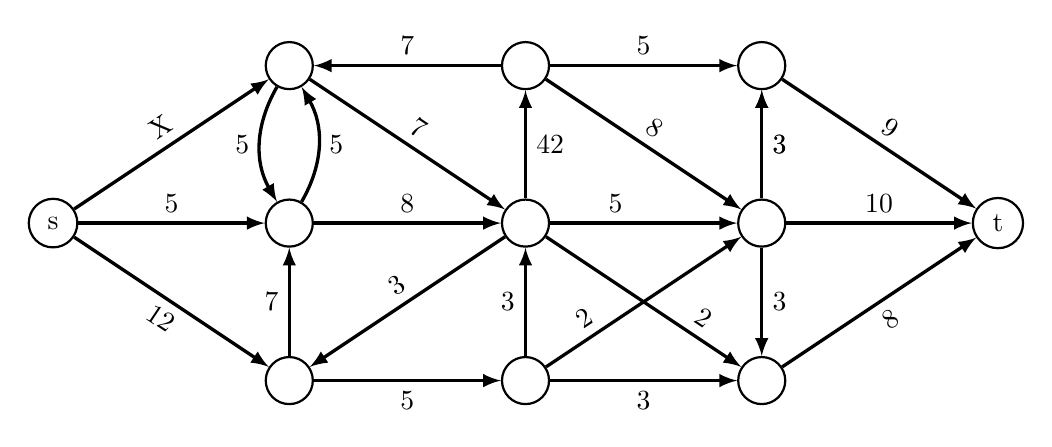
\begin{tikzpicture}[every circle node/.style={
	            draw, 
	            thick,
	            align = center,
	            inner sep=0pt,
                text width=6mm,
	            },
	            >=latex,
	            every path/.style={
                    draw,
                    very thick
                }]
	    
	        \node[circle] (s) at (-1,0) {s};
	        \node[circle] (1) at (2,2) {};
	        \node[circle] (2) at (2,0) {};
	        \node[circle] (3) at (2,-2) {};
	        \node[circle] (4) at (5,2) {};
	        \node[circle] (5) at (5,0) {};
	        \node[circle] (6) at (5,-2) {};
	        \node[circle] (7) at (8,2) {};
	        \node[circle] (8) at (8,0) {};
	        \node[circle] (9) at (8,-2) {};
	        \node[circle] (t) at (11, 0) {t};
	        
	        \draw[->] (s) -- node[sloped, above] {X} (1);
	        \draw[->] (s) -- node[sloped, above] {5} (2);
	        \draw[->] (s) -- node[sloped, below] {12} (3);
	        
	        \draw[->] (1) edge[bend right] node[left] {5} (2);
	        \draw[->] (4) -- node[sloped, above] {7} (1);
	        \draw[->] (1) -- node[sloped, above] {7} (5);
	        
            \draw[->] (3) -- node[left] {7} (2); 
	        \draw[->] (2) edge[bend right] node[right] {5} (1);	 \draw[->] (2) -- node[above] {8} (5);
	        
	        \draw[->] (5) -- node[sloped,above] {3} (3);
	        \draw[->] (3) -- node[below] {5} (6);
	        
	        \draw[->] (4) -- node[above] {5} (7);
	        \draw[->] (4) -- node[sloped, above] {8} (8);
	        \draw[->] (5) -- node[right] {42} (4);
	        
	        \draw[->] (5) -- node[above, pos=.35] {5} (8);
	        \draw[->] (6) -- node[left] {3} (5);
	        \draw[->] (5) -- node[sloped, pos=.75, above] {2} (9);
	        
	        \draw[->] (6) -- node[sloped, pos=.25, above] {2} (8);
	        \draw[->] (6) -- node[below] {3} (9);
	        
	        \draw[->] (8) -- node[right] {3} (7);
	        \draw[->] (8) -- node[right] {3} (9);
	        
	        \draw[->] (8) -- node[right] {3} (7);
	        
	        \draw[->] (7) -- node[sloped, above] {9} (t);
	        \draw[->] (8) -- node[above] {10} (t);
	        \draw[->] (9) -- node[sloped, below] {8} (t);

	    \end{tikzpicture}
	\end{center}

	\begin{enumerate}
	\item \textit{Make a diagram showing the minimum cut corresponding to the maximum flow for $G$ (where $X=0$). Explain in terms of saturated and avoided edges why this is the minimum cut. Give the weight of this cut.}
	
    \begin{center}
	    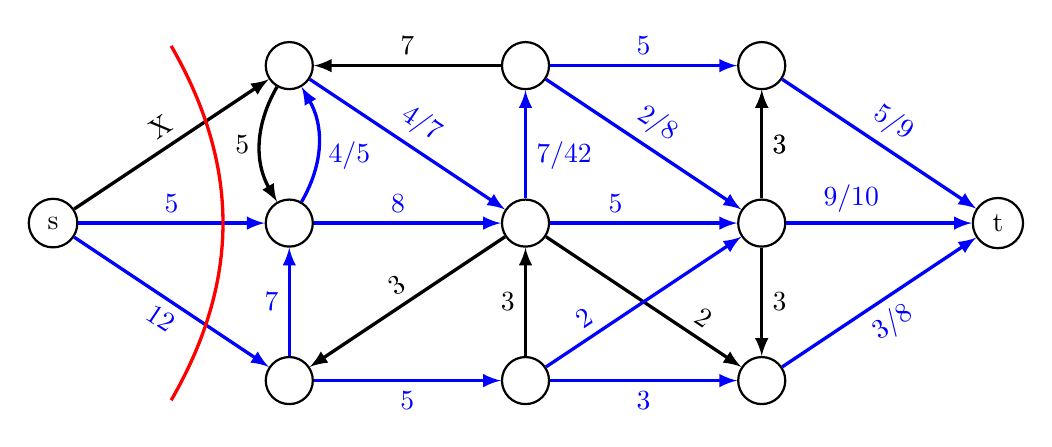
\begin{tikzpicture}[every circle node/.style={
	            draw, 
	            thick,
	            align = center,
	            inner sep=0pt,
                text width=6mm,
	            },
	            >=latex,
	            every path/.style={
                    draw,
                    very thick
                }]
	    
	        \node[circle] (s) at (-1,0) {s};
	        \node[circle] (1) at (2,2) {};
	        \node[circle] (2) at (2,0) {};
	        \node[circle] (3) at (2,-2) {};
	        \node[circle] (4) at (5,2) {};
	        \node[circle] (5) at (5,0) {};
	        \node[circle] (6) at (5,-2) {};
	        \node[circle] (7) at (8,2) {};
	        \node[circle] (8) at (8,0) {};
	        \node[circle] (9) at (8,-2) {};
	        \node[circle] (t) at (11, 0) {t};
	        
	        \draw[->] (s) -- node[sloped, above] {X} (1);
	        \draw[->, blue] (s) -- node[sloped, above] {5} (2);
	        \draw[->, blue] (s) -- node[sloped, below] {12} (3);
	        
	        \draw[->] (1) edge[bend right] node[left] {5} (2);
	        \draw[->] (4) -- node[sloped, above] {7} (1);
	        \draw[->, blue] (1) -- node[sloped, above] {4/7} (5);
	        
            \draw[->, blue] (3) -- node[left] {7} (2); 
	        \draw[->, blue] (2) edge[bend right] node[pos=.4, right] {4/5} (1);	\draw[->, blue] (2) -- node[above, pos=.45] {8} (5);
	        
	        \draw[->] (5) -- node[sloped,above] {3} (3);
	        \draw[->, blue] (3) -- node[below] {5} (6);
	        
	        \draw[->, blue] (4) -- node[above] {5} (7);
	        \draw[->, blue] (4) -- node[sloped, above] {2/8} (8);
	        \draw[->, blue] (5) -- node[pos=.4, right] {7/42} (4);
	        
	        \draw[->, blue] (5) -- node[above, pos=.35] {5} (8);
	        \draw[->] (6) -- node[left] {3} (5);
	        \draw[->] (5) -- node[sloped, pos=.75, above] {2} (9);
	        
	        \draw[->, blue] (6) -- node[sloped, pos=.25, above] {2} (8);
	        \draw[->, blue] (6) -- node[below] {3} (9);
	        
	        \draw[->] (8) -- node[right] {3} (7);
	        \draw[->] (8) -- node[right] {3} (9);
	        
	        \draw[->] (8) -- node[right] {3} (7);
	        
	        \draw[->, blue] (7) -- node[sloped, above] {5/9} (t);
	        \draw[->, blue] (8) -- node[above, pos=.35] {9/10} (t);
	        \draw[->, blue] (9) -- node[sloped, below] {3/8} (t);
	        
	        \draw[red] (0.5,2.25) edge[bend left] (0.5,-2.25);

	    \end{tikzpicture}
	\end{center}
	
	The red line above shows the minimum cut, where all edges under the cut are saturated. Notably, any other potential places for a cut would include either avoided forward edges, or include non-saturated forward edges.
	
	\item \textit{If Hagrid adds the canal $X$, what is the smallest capacity that would maximize the increase in the water flow across the network? Explain.}
	
	    	\begin{center}
	    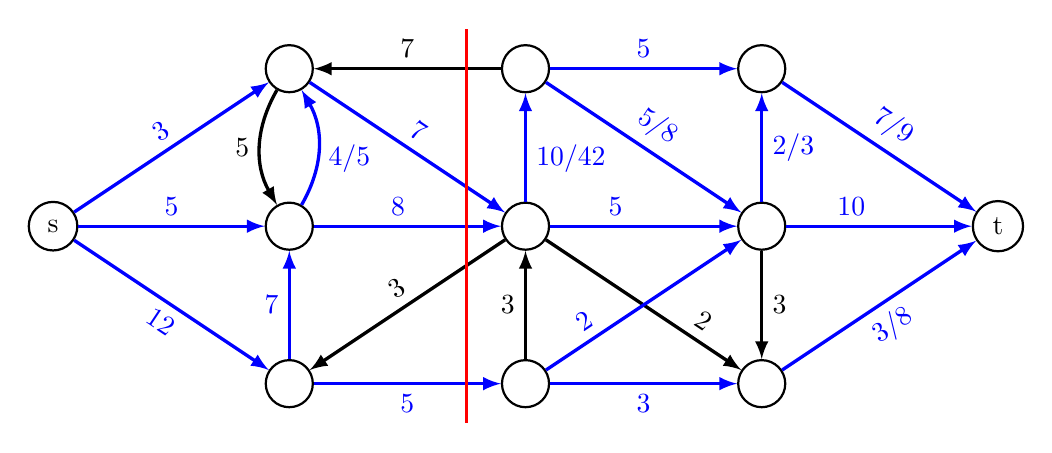
\begin{tikzpicture}[every circle node/.style={
	            draw, 
	            thick,
	            align = center,
	            inner sep=0pt,
                text width=6mm,
	            },
	            >=latex,
	            every path/.style={
                    draw,
                    very thick
                }]
	    
	        \node[circle] (s) at (-1,0) {s};
	        \node[circle] (1) at (2,2) {};
	        \node[circle] (2) at (2,0) {};
	        \node[circle] (3) at (2,-2) {};
	        \node[circle] (4) at (5,2) {};
	        \node[circle] (5) at (5,0) {};
	        \node[circle] (6) at (5,-2) {};
	        \node[circle] (7) at (8,2) {};
	        \node[circle] (8) at (8,0) {};
	        \node[circle] (9) at (8,-2) {};
	        \node[circle] (t) at (11, 0) {t};
	        
	        \draw[->, blue] (s) -- node[sloped, above] {3} (1);
	        \draw[->, blue] (s) -- node[sloped, above] {5} (2);
	        \draw[->, blue] (s) -- node[sloped, below] {12} (3);
	        
	        \draw[->] (1) edge[bend right] node[left] {5} (2);
	        \draw[->] (4) -- node[sloped, above] {7} (1);
	        \draw[->, blue] (1) -- node[sloped, above] {7} (5);
	        
            \draw[->, blue] (3) -- node[left] {7} (2); 
	        \draw[->, blue] (2) edge[bend right] node[pos=.4, right] {4/5} (1);	\draw[->, blue] (2) -- node[above, pos=.45] {8} (5);
	        
	        \draw[->] (5) -- node[sloped,above] {3} (3);
	        \draw[->, blue] (3) -- node[below] {5} (6);
	        
	        \draw[->, blue] (4) -- node[above] {5} (7);
	        \draw[->, blue] (4) -- node[sloped, above] {5/8} (8);
	        \draw[->, blue] (5) -- node[pos=.4, right] {10/42} (4);
	        
	        \draw[->, blue] (5) -- node[above, pos=.35] {5} (8);
	        \draw[->] (6) -- node[left] {3} (5);
	        \draw[->] (5) -- node[sloped, pos=.75, above] {2} (9);
	        
	        \draw[->, blue] (6) -- node[sloped, pos=.25, above] {2} (8);
	        \draw[->, blue] (6) -- node[below] {3} (9);
	        
	        \draw[->] (8) -- node[right] {3} (9);
	        
	        \draw[->, blue] (8) -- node[right] {2/3} (7);
	        
	        \draw[->, blue] (7) -- node[sloped, above] {7/9} (t);
	        \draw[->, blue] (8) -- node[above, pos=.35] {10} (t);
	        \draw[->, blue] (9) -- node[sloped, below] {3/8} (t);
	        
	        \draw[red] (4.25,2.5) edge (4.25,-2.5);

	    \end{tikzpicture}
	\end{center}
	
	X can be at most 3, as that is what saturates the next "layer" of forward pipes, as shown above. The red line above is a possible minimum cut while X is 3, and the only minimum cut if X is greater than 3. 
	
	\item \textit{Describe how Hagrid could use a min-cut/max-flow algorithm to decide what capacity $X$ should be used for an arbitrary graph $G=(V,E)$ and arbitrary proposed edge $(u,v)\not\in E$ with capacity $X$.}
	
	Using a min-cut/max-flow algorithm, Hagrid could find the min-cut and then add an edge with infinite capacity. Then, Hagrid could find the min-cut on the augmented graph, find the capacity of that min-cut, and reduce the capacity of the added edge until there are two possible min-cuts. 
	
	\end{enumerate}

    \newpage
	\item \textit{(30 pts total) After a brilliant prank goes awry, your wizard friends Fred and George Weasley have bitter argument. You intervene to keep the peace and they agree to stay away from each other, for the time being. In particular, they have agreed that when navigating the halls of Hogwarts, each will not walk on any section of stone that the other wizard has stepped on that day. The wizards have no problem with their paths crossing at an intersection. The problem, however, is that they both still need to get to the Great Hall each day to eat. Fortunately, both the Gryffindor house entrance $s$ and Great Hall $t$ are at intersections. You have a map of Hogwarts' hallways and their intersections, on which the Gryffindor entrance and the Great Hall are marked.}
	
	\textit{Your task is to determine whether there exists a pair of edge disjoint paths that would allow your friends to both get from $s$ to $t$. Explain how to represent the problem as a graph $G$ for which a straight-forward application of a max-flow/min-cut algorithm will yield the answer, and the paths.}\\
	
% 	{\sf dibs -G}
	
	This problem can be turned into a max-flow/min-cut problem by creating a graph from the map of Hogwarts. This graph has each intersection as the nodes of the graph, and each hallway as an undirected edge with weight 1. If we mark the Gryffindor house entrance as the source $s$ and the Great Hall as the sink $t$, then we can apply the max-flow/min-cut algorithm to see if we can push a max flow of $2$ through the graph.\\
	
	If the max flow is $2$ or greater, then that means since each edge has weight $1$, there are at least two paths from $s$ to $t$ which do not share edges. Each of these paths will be pushing through $1$ unit of flow, so if each Weasley brother takes one of these paths, they will keep the peace.\\
	
	\newpage
	\item \textit{(10 pts extra credit) Preparing for a big end-of-semester party at Hogwarts, you crack open the Gryffindor cellar and count $n$ bottles of fine drink. Dumbledore has previously warned you that exactly $k$ of these bottles have been poisoned (he wouldn't go into detail as to how exactly this came to be), and consuming poisoned drink will result in an unpleasant death. The party starts in one hour, and you do not want to poison any of your guests.}
	
	\textit{Luckily, a family of $\ell$ docile rats occupies a corner of the cellar, and they have graciously volunteered to be test subjects for identifying the poisoned bottles. Let $\ell=o(n)$ and $k=1$, and assume it takes just under one hour for poisoned drink to kill a rat. (Hence, you only get one shot at solving this problem.)}
	
	\textit{Describe a scheme by which you can feed the drink to rats and identify with complete certainty the poisoned bottle, prove that the scheme is correct, and give a tight bound on the number of rats $\ell$ necessary to solve the problem.}
	
	\textit{Dumbledore's hint: 1010101111}\footnote{Fortunately for Dumbledore, a king of the ancient times encountered a similar problem, and posted it on Reddit: {\tt https://www.reddit.com/r/riddles/comments/16b5il/}}\\
	
% 	{\sf dibs -G}

    Since $k = 1$, there is an elegant solution that involves using a binary labeling system. We label the bottles from $1$ to $n$ in binary, and then assign each valiant rat a digit. For example, if there were $16$ bottles of fine drink, we would label them like $0000$, $0001$, $0010$, $0011$, ..., $1111$ so that each bottle has a unique binary representation. Then, we have four rats: one drinking a drop from each of the bottles with $1$ in the leftmost digit, one drinking a drop from each of the bottles with a $1$ in the second digit, and so on. After an hour, we see which rats have died and recreate the number: if a digit's rat died, then it is $1$. Otherwise, it is $0$. From there we have constructed a unique binary number that tells us exactly which bottle has been poisoned.\\
    
    We require exactly $\ell = \lceil\lg n\rceil$ rats for a solution to this problem, since to represent a number $n$ in binary, we need $\lceil \lg n \rceil$ digits.

\end{enumerate}

\end{document}